\documentclass[12pt,a4paper,titlepage,twoside]{report}
\usepackage[T1]{fontenc}
\usepackage[english, spanish]{babel}
\usepackage[utf8]{inputenc}
\usepackage{lmodern}
\usepackage{graphicx}
\usepackage{csquotes}
\usepackage{xcolor}
\usepackage{url}
\usepackage[backend=biber,style=alphabetic,
sorting=ynt]{biblatex}
\addbibresource{biblio.bib}
% http://tug.ctan.org/tex-archive/macros/latex/contrib/fancyhdr/
\usepackage{fancyhdr}
\pagestyle{fancy}
\fancyhf{}
\fancyhead[LE,RO]{\nouppercase \rightmark}
\fancyhead[LO,RE]{\nouppercase \leftmark}
\fancyfoot[C]{\thepage}

%Carpeta de imagenes
\graphicspath{ {img/}}

\newcommand{\Keywords}[1]{\vfill\noindent{\small{\em Palabras clave}: #1}}
\definecolor{grisclar}{gray}{0.5}
\definecolor{grisfosc}{gray}{0.25}

% Editar con los datos correspondientes
\newcommand{\titulo}{Diseño e implementación de un Cluster de virtualización en alta disponibilidad para los servicios de emergencias del Consorcio Provincial de Bomberos de Valencia}
\newcommand{\titulacion}{Ingeniería en Informática}
\newcommand{\autor}{María Alexandra Hermosilla Semikina}
\newcommand{\director}{Alberto Conejero}

\title{\titulo}
\author{\autor}

\begin{document}
% Portada basada en el ejemplo de:
% http://en.wikibooks.org/wiki/LaTeX/Title_Creation

\begin{titlepage}
\begin{center}

% Logos UPV y ETSINF
\begin{minipage}{0.49\linewidth}
\begin{flushleft}

\includegraphics[height=1.5cm]{./logo-upv}
\end{flushleft}
\end{minipage}
\begin{minipage}{0.49\linewidth}
\begin{flushright}

\includegraphics[height=1.5cm]{./logo-etsinf}
\end{flushright}
\end{minipage}

\vspace{2cm}

\begin{color}{grisfosc}
\large
Escola Tècnica Superior d'Enginyeria Informàtica\\[0.2cm]
Universitat Politècnica de València\\[1.9cm]
\end{color}

% Título del proyecto y titulación
{\LARGE \bfseries \titulo}\\[1.5cm]
\textsc{\large Proyecto Final de Carrera}\\[0.4cm]
\textcolor{grisclar}{\large\titulacion}\\[5.0cm]

% Autor, director y fecha
\begin{flushright} \large
\emph{Autor:} \autor\\[0.4cm]
\emph{Director:} \director\\[0.6cm]
\today
\end{flushright}

%\vfill
% Bottom of the page
%{\large \today}

\end{center}

\end{titlepage}


\begin{abstract}
Este proyecto nació a partir de la necesidad de un cluster de virtualización que estuviera en alta disponibilidad para albergar las herramientas que utiliza el Consorcio Provincial de Bomberos de Valencia tanto para los servicios de emergencia como los servicios internos. 
El Consorcio Provincial de Bomberos de Valencia ha ido aumentando los servicios que presta a nivel interno como a nivel operativo en los servicios de emergencia, consecuentemente es necesario ampliar su infraestructura de virtualización como adaptarse al nuevo hardware que se ha incorporado a la infraestructura ya existente.
Para ello, se ha construido un cluster de virtualización basado en tecnologías como Xen, corosync y pacemaker.

\Keywords{Virtualización, HA, Alta disponibilidad, Xen, Servicios de emergencia, Cluster, Debian, Linux,Corosync, Pacemaker, ocfs2, Máquina Virtual,GNU}
\end{abstract}

\tableofcontents

\chapter{Introducción}
En la administración de sistemas siempre ha habido una gran problemática alrededor de la optimización de los recurso. Estos recursos no solo son a nivel de hardware, si no que también a nivel de refrigeración, consumo eléctrico y espacio, entre otros factores. El coste del mantenimiento era extremadamente elevado para entidades que disponían de infraestructuras informáticas muy grandes, ya que no solo era necesario disponer de repuestos, si no también de un elevado número de personal dedicado a esta labor.
\par
Desde la llegada de la virtualización, la informática ha sufrido una gran revolución en este aspecto. La virtualización consiste en una capa de software que corre en un sistema operativo que crea una abstracción entre el hardware y el software a ejecutar. Para este software, esta capa, es totalmente transparente, ya que ve los mismos recursos de hardware que vería un sistema operativo nativo. El software puede ser cualquier recurso que necesitemos como una computadora, sistema operativo, dispositivo de almacenamiento, aplicaciones o redes. Esto permite que, en caso de fallo de hardware, este software se pueda trasladar a otro hardware que corra la misma capa de abstracción y el software no se percate del cambio y siga funcionando sin problemas. 
\par
Como se puede apreciar, la virtualización presente una serie de ventajas respecto a las infraestructuras físicas. De estas ventajas se puede destacar las siguientes:
\begin{itemize}
\item \textbf{Aislamiento:} Cada máquina virtual es independiente una de la otra y del hypervisor. Por lo que si una de ellas falla, no afecta a las demás como tampoco al hypervisor.
\item \textbf{Seguridad:} En caso de lograr acceso privilegiado a una de estas máquinas virtuales, sólo se obtendría acceso a dicha máquina, dejando intactas el resto de máquinas y  el hypervisor donde reside dicha máquina virtual.
\item \textbf{Flexibilidad:} Las máquinas virtuales, al ser software, se les puede asignar los recursos necesarios (CPU, RAM, HDD...) sin necesidad de comprar un hardware concreto para ellas. Esto permite ampliarlas en un momento de uso alto de recursos o quitarlos cuando no son necesarios.
\item \textbf{Agilidad:} La puesta en marcha de una máquina virtual suele ser un proceso sencillo. Se puede hacer a través de rellenar un fichero con los recursos necesarios o a través de un asistente de creación. Con ello, una máquina virtual está funcionando en cuestión de minutos.
\item \textbf{Portabilidad:} El hecho de que las máquinas virtuales sean un par de ficheros,permite cambiarla de hypervisor o hardware sin gran problema. Solo es mover unos ficheros y volver a ejecutar la máquina.
\end{itemize}
\par 
Todas estas características son las que se busca en una infraestructura donde el número de servicios prestados es alto y deben estar en alta disponibilidad. Este es el caso del Consorcio Provincial de Bomberos de Valencia. Donde el número de servicios de información prestados son elevados y diversos. Algunos de ellos es necesario que estén operativos las 24 del día. 
\par
En octubre de 2012 accedí al Consorcio Provincial de Bomberos de Valencia como becaria para realizar las labores de apoyo en las áreas de administración de sistemas y helpdesk. Los primeros meses de la beca se me formó en las tecnologías usadas en la infraestructura utilizada para dar servicio a la sede central y a los diferentes parques que forman el Consorcio. Posteriormente y ante la urgencia de desplegar nuevos servicios, se me asigno al proyecto de la creación de un nuevo cluster de virtualización sobre el hardware Unified Computing System (UCS) de Cisco con cuatro blades listos para la instalación y configuración del cluster.


\section{Consorcio Provincial de Bomberos de Valencia}
Durante los años 60, gracias a la expansión económica, la provincia de Valencia sufrió una gran transformación socioeconómica que conllevo a un aumento de población e industrialización. Estos factores influyeron de manera notoria en el aumento del riesgo y en la demanda de los servicios de emergencias.Por este motivo, en 1982 se constituyeron los primeros servicios de emergencias en la provincia de Valencia en forma de Consorcios Comarcales. Se agruparon en mancomunidades a varios municipios por comarcas con el objetivo de facilitar la prestación de este servicio. De esta forma, se crearon 7 consorcios comarcales con la ayuda de la Diputación de Valencia: Horta Nord, Horta Sud, Camp de Morvedre, Ribera Baixa, Ribera Alta-Valldigna, La Safor y La Costera.
\par
Esta diseminación dejó patente las carencias y problemas de organización y coordinación. Por este motivo, el 31 de octubre de 1986 se constituye un único órgano provincial, el Consorcio Provincial de Bomberos de Valencia, tras la aprobación de sus Estatutos por la Generalitat, la Diputación de Valencia y los 132 municipios que se integraron en él.
\par
Actualmente, el Consorcio cubre una superficie de 10.671,48 kilómetros cuadrados, 5.819 kilómetros cuadrados de masa forestal, más de 3.000 kilómetros de carreteras, 1.700.829 vehículos y cerca de 184.483 empresas contabilizadas en la provincia de Valencia. Como también el número de pueblos que se encuentran adheridos a esta mancomunidad a ascendido a 265 pueblos. Para realizar su labor de forma eficaz el Consorcio esta formado por 17 parques profesiones, 7 parques voluntarios y una sede central situada en la ciudad de Valencia. La distribución de los parques se agrupa en 6 zonas que cubre la totalidad de la provincia. Cada zona cuenta con un parque principal y al menos un parque auxiliar, dependiendo de la zona a cubrir. Algunas zonas cuentan con parques de voluntarios para completar la cobertura.
\par
En todo momento y a lo largo de toda la provincia se encuentran de guardia más de 100 bomberos que son capaces de atender el 81'14 por ciento de los riesgos que presentan las actividades por Incendios, Salvamentos y Prevenciones por Asistencia Técnica, en menos de 10 minutos.Se atiende el 98,03 por ciento si el tiempo de respuesta lo fijamos hasta los 20 minutos.
El promedio anual de servicios realizados asciende a 14000, pero cada sigue en aumento. Aunque su principal labor consiste en la extinción de incendios urbanos, industriales y forestales, también se realizan rescates de de automovilistas atrapados en accidentes de tráfico que ha ido en aumento a lo largo de los últimos años. \cite{web1} \cite{web2}
\section{Servicios de información que se prestan y su taxonomía}
En una entidad como el Consorcio es fácil encontrar una gran variedad de servicios que se presten a nivel interno como también de cara al ciudadano. Todos estos servicios se pueden clasificar de diferentes manera, pero en este caso se pueden aplicar dos tipos de clasificaciones. La primera se basa en a quién están dirigidos los servicios. En este caso, se pueden encontrar dos categorías principales: el ciudadano y el trabajador del centro. De cara al ciudadano, se dispone de portales web, a través de los cuales, pueden obtener toda la información necesaria sobre el consorcio y los parques de bomberos. 

A nivel del trabajador del Consorcio, el número de servicios de la información es considerable. No se hablará en detalle de los servicios, ya que no es el propósito de este documento, pero se describirá las diferentes categorías que los alberga. Estos servicios a nivel interno del departamento de informática se han catalogado usando como ejemplo el catalogo de servicios usado en la universidad Stanford \cite{Stanford}, California. Esta clasificación esta basada en las buenas practicas para la administración de los servicios informáticos ITIL \cite{ITIL}.

\begin{itemize}
\item \textbf{Cuentas de usuario:} Es necesario entender que existen varios tipos de usuario, ya que no todos necesitan tener el mismo nivel de seguridad ni de acceso a los recursos. Por ejemplo, un bombero no necesita tener el acceso a los recursos y servicios del departamento de recursos humanos, solo necesitará poder comunicarse de manera telemática con dicho departamento. Por lo tanto, se han implementado diferentes tipos de cuentas, las cuales, permiten tener acceso a diferentes niveles de seguridad y servicios. 
\item \textbf{Email y Colaboración:} Para poder agilizar la comunicación tanto interna como externa se dispone de servicio propio de correo. Todo empleado del Consorcio dispone de una cuenta ya que la mayor parte de la comunicación interna se realiza a través de dicho correo. Por otra parte, existe una plataforma colaborativa de trabajo para que aquellos unidades de trabajo que requieran del intercambio de documentación e información puedan realizarlo. Esta plataforma esta basada en Alfresco \cite{alfresco}, la cual es un gestor de documentos y de procesos de negocio.  Para poder acceder a esta plataforma es necesario disponer de una cuenta de Active Directory.
\item \textbf{Aplicaciones Corporativas:} En esta categoría se engloban todas las aplicaciones que se usen a diario para la realización de las labores diarias, tanto a nivel administrativo como también a nivel operativo. Parte de estas aplicaciones han sido hechas por terceros y su soporte depende de ellos. Otra parte de las aplicaciones se han realizado internamente desde el departamento para cubrir necesidades muy concretas.
\item \textbf{Redes:} Esta categoría engloba toda la infraestructura de redes a través de la cual se sirven todos los servicios. En ella incluye todas las redes físicas,las redes virtuales, wifi, VPN, etc. Al disponer de diferentes sedes a lo largo de toda la provincia de Valencia, es necesario disponer de una infraestructura para distribuir los servicios a los 24 parques de bomberos, incluyendo los voluntarios, y a la sede central. Por otra parte, también es necesario destacar que determinados servicios deben ser proporcionados en los puestos de mando avanzado cuando existe un incendio de gran envergadura por lo que es necesario disponer de conexión a los servicios del consorcio desde cualquier punto de la provincia. Esto se logra mediante varias conexiones de internet a través de 3G/4G y redes VPN.
\item \textbf{Servidores y Almacenamiento:} Todos los servicios deben residir en alguna parte, por lo que es necesario un ordenador físico o una máquina virtual que los sirva, como también la gran cantidad de datos que es necesario almacenar y servir en cualquier momento. En estos momento, disponemos de aproximadamente 32 máquinas virtuales y 8 físicas que actúan como servidores de dichos servicios. Por otra parte, para almacenar toda la información, incluyendo las propias máquinas virtuales, se dispone de 2 cabinas de almacenamiento. Estas cabinas se comunican directamente con los hypervisores como también con las máquinas virtuales. 
\item \textbf{Seguridad:} Como cualquier entidad tanto pública como privada requiere de protección de la infraestructura como también de la información que circula por ella. Por ello, se han desplegado diferentes servicios. Uno de los servicios principales es el cortafuegos, basado en el pfsense \cite{pfsense}. El cual, no solo actúa de cortafuegos para toda la infraestructura, sino también como router entre las diferentes redes de las que se disponen y a las redes externas que nos conectamos. Adicionalmente, toda la infraestructura esta detrás de los cortafuegos de la Generalitat Valenciana, gestionado por el CSIRT-CV \cite{csirtcv} por lo cual, el primer filtro se realiza a través de ellos. Pero estas medidas no son suficientes, por lo que en cada ordenador con sistema Microsoft Windows, se dispone de un antivirus, pero evitar las amenazas de virus de forma directa. A nivel de usuario, se han ido adaptando y creando diferentes políticas de seguridad para la prevención de los diferentes tipos de amenazas disponibles. Por otro lado, es necesario poder monitorizar la seguridad en tiempo real. Para ello, se utiliza un sistema de gestión de la información de seguridad y administrador de eventos, OSSIM \cite{ossim}. Mediante este sistema, tenemos información completa de las vulnerabilidades, amenazas y ataques en tiempo real a lo largo de toda la infraestructura del consorcio.
\item \textbf{Soporte al Desktop:} Para poder atender correctamente al usuario, y teniendo en cuenta las múltiples ubicaciones y tipos de usuarios, es necesario disponer de herramientas adecuadas para esta labor. Para ello, se utilizan distintas herramientas de control remoto, un sistema de gestión de incidencias, manuales de usuario para las diferentes aplicaciones desplegadas y asistencia por teléfono y correo electrónico.
\item \textbf{Servicios web:} Algunos de los servicios, para facilitar el acceso a ellos, se sirven en formato web. Estos servicios son los portales web, tanto las webs públicas como también determinadas aplicaciones. El correo electrónico también dispone de su plataforma web para facilitar el acceso desde cualquier parte, sin necesidad de algún cliente de correo especifico. 
\item \textbf{Certificación digital:} El departamento de informática no es ninguna autoridad certificadora, pero realizan las labores necesarias para que los usuarios puedan solicitarlo. Estos certificados son utilizados sobre todo para la comunicación entre las diferentes administraciones públicas.
\item \textbf{Gestión de TI:} A nivel interno del departamento de informática, es necesario poder gestionar los dispositivos y sistemas, por lo que se usan algunas herramientas especificas para ello. Una de estas estas aplicaciones es el UCS Manager, responsable de la gestión del chasis, blades y Fabric Interconnect
\item \textbf{Otros servicios:} En esta categoría se pueden encontrar algunos servicios específicos que no se pueden clasificar en las categorías anteriores. Entre ellos, se encuentra el servidor cartográfico el cual es utilizado por parte del cuerpo operativo para las labores de prevención, formación y extinción de incendios. 
\end{itemize}

\chapter{Antecedentes}
El Consorcio cuenta en estos momentos con un personal que asciende a más de 800 personas, entre las cuales no solo se encuentra el personal operativo, sino también de personal administrativo. Cada uno de estos dos grupos de usuarios requiere de herramientas diferentes y especializadas para su labor. 
\par
Para el personal operativo es necesario que los servicios usados para su labor estén operativos siempre y poder acceder a ellos en cualquier momento y lugar. Por una parte, el Consorcio es el responsable de recibir los servicios solicitados por parte del 112 de la Generalitat Valenciana que requieran la intervención de los bomberos. Sin embargo, esta parte esta gestionada por parte del propio 112 GVA. Para la gestión del servicio a prestar sí se usa un software propio que esta gestionado internamente. Este servicio es usado no solo por parte de los operadores, sino que también por parte de todo el personal operativo. Esto quiere decir que tiene que estar disponible desde cualquier parque de bomberos de la provincia de Valencia, incluyendo los parques de voluntarios.
\par
Por otra parte, el personal administrativo es el que más servicios requiere, ya que son los responsables de toda la gestión de la organización. Esto quiere decir, que a pesar de ser el grupo minoritario, son los que más recursos necesitan para realizar su labor.
\section{Infraestructura previa}
Para mantener todos los servicios que se prestan, se disponía de una infraestructura formada por dos servidores HP Proliant DL380 G5 y una cabina HP EVA 4100 Fiber Channel. Sus características son las siguientes:
\begin{itemize}
    \item Procesador: Intel Pentium Xeon QuadCore 2.3 GHz
    \item RAM: 16GB
    \item Tarjeta de red: Broadcom NetXtreme 57xx Gigabit Controller
    \item Tarjeta de red: Intel 82567LF Gigabit Network Connection
    \item Tarjeta de red: HBA FC 4Gbps PCI-e
    \item Tarjeta de red: HP ILO
    \item Disco duro: 376596-001 HP 360GB 3G 10K 2.5" SP SAS
    \item Disco duro: 507284-001 HP 300GB 2.5" SAS 10K
\end{itemize}

\par Como se puede ver por las características, los servidores no tienen un almacenamiento amplio ya que sirven las máquinas desde la cabina de almacenamiento. Esto permite que los servidores sean mucho más ligeros y elimina la limitación física de los discos duros, pudiendo servir espacios mucho más amplios.
%meter el diagrama de la antigua configuración.
\begin{figure}[h]
\caption{Diagrama del cluster anterior}
\centering
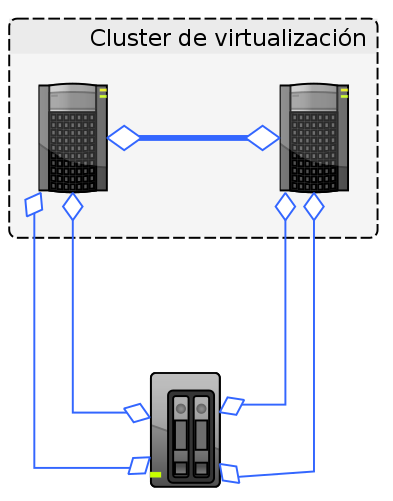
\includegraphics[scale=0.5]{cluster-anterior}
\end{figure}
\par
Como se puede apreciar en el diagrama, cada servidor del cluster se conecta a la cabina por dos conexiones de fibra óptica. Estas conexiones permiten asegurar que siempre haya acceso desde el servidor. Sin embargo, no se tiene acceso a toda la cabina, sino al volumen asignado para almacenar y servir las máquinas virtuales. Por otra parte, algunas maquinas virtuales necesitan tener acceso a volúmenes propios que pueden estar en esta cabina o en otra. 
\par
Los servidores del cluster estaban basados en la versión de largo mantenimiento (LTS) del servidor de Ubuntu \cite{ubuntu}. Esto permite que los servidores siempre estén actualizados y no haya agujeros de seguridad.

\section{Nuevos servicios a prestar}
Al intentar adaptarse a la nueva gestión electrónica que se requiere en la administración pública, ha sido necesario incluir nuevos productos para dar estos nuevos servicios. Para ello, es necesario que algunos de los servicios exisitentes pasen a estar interconectados entre ellos como también actualizarse a productos que se ajusten mejor a las necesidades del Consorcio. 
\par
Los nuevos servicios que se incluirán tras el cambio del cluster son:
\begin{itemize}
    \item Gestión de la contabilidad
    \item Gestión de recursos humanos
    \item Portal del ciudadano
    \item Portal de transparencia
\end{itemize}
Todos los servicios, a excepción del Portal de transparencia, requieren de máquinas virtuales muy potentes con lo que el cluster existente no cumple con los requisitos de memoria, cores ni espacio en el volumen de almacenamiento para albergar estas máquinas y las ya existentes. Por otro lado, para el Portal de transparencia aun no se han establecido los requisitos del software por lo que queda pendiente de implementar.
\par
Para los servicios que sí se van a implementar en esta fase, se requiere de 7 máquinas virtuales con las siguientes características:
\begin{itemize}
    \item 2 Máquinas virtuales con:
    \begin{itemize}
        \item RAM 4GB
        \item vCPU: 1
    \end{itemize}
    \item 1 Máquina virtual con:
    \begin{itemize}
        \item RAM 4GB
        \item vCPU: 2
    \end{itemize}
    \item 2 Máquinas virtuales con:
    \begin{itemize}
        \item RAM 16GB
        \item vCPU: 4
    \end{itemize}
    \item 2 Máquinas virtuales con:
    \begin{itemize}
        \item RAM 6GB
        \item vCPU: 2
    \end{itemize}
    
\end{itemize}

Estas máquinas se separan en dos grupos, 6 máquinas con sistema operativo Microsoft Windows Server 2012 y una con una Ubuntu 14.4 LTS.
Como se puede apreciar, son máquinas con unos requerimientos muy altos. Con lo cual, no se pueden crear en el cluster actual debido a la falta de RAM y vCPU. Debido a esto y a otros proyectos que todavía no se han definido sus requisitos de hardware, es necesario implementar el nuevo cluster, el cual, sí dispone de todos los recursos necesarios para los proyectos actuales como para futuros.
\par
A nivel de funcionamiento de estas máquinas virtuales, es necesario que 4 de ellas estén separadas por parejas en los hypervisores para asegurar la alta disponibilidad. Esto es imposible en el cluster actual. Por otra parte, 6 de las 7 máquinas virtuales están basadas en el sistema operativo de Microsoft Windows 2012.
\section{Requisitos de la solución}

Para la nueva solución es necesario definir los requisitos para una completa integración con la infraestructura.
\begin{itemize}
%Revisar el primer punto
    \item Debe ser compatible con la infraestructura de Cisco UCS, los blades modelo B200M y los Factor Interconnect.
    \item Es necesario que el almacenamiento sea distribuido por SCSI y compartido entre todos los hypervisores. Por una parte, habrá un almacenamiento desde el cual se servirán las máquinas virtuales y, por otra parte, cada máquina es posible que requiera de un almacenamiento adicional para su uso.
    \item No debe suponer un problema la migración de las máquinas virtuales desde la vieja plataforma a la nueva.
    \item Los nodos Hypervisores deben servir las máquinas en alta disponibilidad. Esto quiere decir que si uno de los nodos cae, el resto asume sus máquinas virtuales y no se interrumpen los servicios prestados por el nodo caído.
    \item Los hypervisores administrarán 7 redes virtuales para que las máquinas virtuales estén ubicadas en la red según convenga.
    \item Capaz de ejecutar las máquinas virtuales que actualmente se están usando y las nuevas.
    \item No debe suponer ninguna inversión. No se dispone de presupuesto para la implementación de una solución para virtualización.
\end{itemize}
%compatible con los ucs b200m
%solución que sea sea compatible con el almacenamiento compartido por scsi
%Compatibilidad con Xen o al menos que la migración de una plataforma a otra no sea traumatica
\chapter{Resumen de alternativas y criterios de selección}
\section{Criterios de selección}
A la hora de seleccionar la solución adecuada para la infraestructura, es necesario basarse en los requisitos de la solución vistos anteriormente.
\section{Proxmox Virtual Environment}
Esta solución proporciona una instalación integrada en un solo paquete desde el sistema operativo, pasando por la solución de virtualización hasta la gestión del nodo. 

%Sistema Operativo entero
%Uso de dos tecnologias diferentes para la virtualización
%Gestión 
El mayor problema que se plantea con Proxmox es que para las máquinas virtuales Microsoft Windows Server 2012
%La empresa Proxmox Server Solutions GmbH es un proyecto que se inició en 2005, pero su producto principal, %el entorno de virtualización, no empezó hasta el año 2008. Este entorno utiliza dos tecnologías diferentes %de virtualización. La primera, enfocada para los sistemas GNU/Linux, basada en OpenVZ. OpenVZ se basa en %contenedores que permite ejecutar múltiples instancias del mismo sistema operativo aislados denominados %Servidores Privados Virtuales (VPS, siglas en inglés). Cada contenedor tiene sus propias archivos y %aplicaciones, usuarios y dispositivos. Todos estos contenedores comparten el mismo kernel
\section{CloudStack}
\section{OpenStack}
OpenStack esta enfocado en el despliegue rápido de máquinas y bajo petición.

Para implementar la opción de OpenStack es necesario adaptar los diferentes componentes de la que esta compuesta a la infraestructura existente. Para ello sería necesario instalar tanto el Nova y el Neoutron en todos los hypervisores para que cada hypervisor pueda gestionar las redes de manera independiente y no se cree un cuello de botella en un solo nodo. 
\section{VMware vSphere}

Esta solución en la fase de análisis se descarta de inmediato. El motivo de su descarte es el coste de la solución, ya que no se dispone de presupuesto para ello. Es cierto que esta solución es de las mejores, pero su coste imposibilita su implantación.
\section{Xen + Pacemaker + Corosync}

\chapter{Implementación de la solución seleccionada}
%Introducción de cómo se realizo
\par A lo largo de este capítulo se explicará el proceso que se ha seguido para la instalación y configuración del los hypervisores. Los cuatro hypervisores son idénticos, por lo que solo se explicará las diferencias entre ellos. 
\par Para preservar la seguridad de la entidad, los datos expuestos aquí no son reales.
\section{Instalación del sistema operativo}
El sistema operativo seleccionado como base ha sido GNU/Debian en su versión estable, la cual, se encontraba en un su release Wheezy, versión 7. Es una instalaci
\section{Instalación y configuración del cliente NTP}
\section{Instalación del hypervisor Xen}
\section{Configuración de la las interfaces y las VLANs}
\section{Instalación y configuración de OpenSwitch}
\section{Instalación del multipath}

%Separar en pasos y resolución de las problemáticas aparecidas
\chapter{Resultados y conclusiones}
%Posibles mejoras
%Posibles lineas de investigación
\chapter{Anexos}
%Ficheros de configuración

%\chapter{Bibliografía}
\nocite{*}
\printbibliography

\end{document}